% Kile - graf. editor
\documentclass[12pt,a4paper]{article}
% File il2code.tex (original name extcode.tex changed in August 1996) does:
%  (0) sets \czech, \slovak to ISO-8859-2 encoded hyphen-pattern numbers,
%  (1) sets \catcode, \l/uccode for characters (code ISO-8859-2),
%  (2) defines \csaccents for new behavior of \v, \', etc (code ISO-8859-2),
%  (3) defines some \sequences for special cs-fonts characters.
%
% Created by Petr Olsak <olsak@math.feld.cvut.cz>,        April, 1995
% September 1996: Better definition of \clqq and friends and \ogonek.
% February 2000: The feature (0) added.

%\message{Font encoding set to ISO-8859-2.}

%% (0) \czech, \slovak. You can use \chyph, \shyph after this file is loaded.
\ifx\iltwoczech\undefined \else
  \czech=\iltwoczech  \slovak=\iltwoslovak
\fi

%% (1) \catcode, \lccode, \uccode.
\catcode225=11 \lccode225=225 \uccode225=193 % a-acute
\catcode193=11 \lccode193=225 \uccode193=193 % A-acute
\catcode228=11 \lccode228=228 \uccode228=196 % a-diaeresis
\catcode196=11 \lccode196=228 \uccode196=196 % A-diaeresis
\catcode232=11 \lccode232=232 \uccode232=200 % c-caron
\catcode200=11 \lccode200=232 \uccode200=200 % C-caron
\catcode239=11 \lccode239=239 \uccode239=207 % d-caron
\catcode207=11 \lccode207=239 \uccode207=207 % D-caron
\catcode233=11 \lccode233=233 \uccode233=201 % e-acute
\catcode201=11 \lccode201=233 \uccode201=201 % E-acute
\catcode236=11 \lccode236=236 \uccode236=204 % e-caron
\catcode204=11 \lccode204=236 \uccode204=204 % E-caron
\catcode237=11 \lccode237=237 \uccode237=205 % i-acute
\catcode205=11 \lccode205=237 \uccode205=205 % I-acute
\catcode229=11 \lccode229=229 \uccode229=197 % l-acute
\catcode197=11 \lccode197=229 \uccode197=197 % L-acute
\catcode181=11 \lccode181=181 \uccode181=165 % l-caron
\catcode165=11 \lccode165=181 \uccode165=165 % L-caron
\catcode242=11 \lccode242=242 \uccode242=210 % n-caron
\catcode210=11 \lccode210=242 \uccode210=210 % N-caron
\catcode243=11 \lccode243=243 \uccode243=211 % o-acute
\catcode211=11 \lccode211=243 \uccode211=211 % O-acute
\catcode244=11 \lccode244=244 \uccode244=212 % o-circumflex
\catcode212=11 \lccode212=244 \uccode212=212 % O-circumflex
\catcode246=11 \lccode246=246 \uccode246=214 % o-diaeresis
\catcode214=11 \lccode214=246 \uccode214=214 % O-diaeresis
\catcode224=11 \lccode224=224 \uccode224=192 % r-acute
\catcode192=11 \lccode192=224 \uccode192=192 % R-acute
\catcode248=11 \lccode248=248 \uccode248=216 % r-caron
\catcode216=11 \lccode216=248 \uccode216=216 % R-caron
\catcode185=11 \lccode185=185 \uccode185=169 % s-caron
\catcode169=11 \lccode169=185 \uccode169=169 % S-caron
\catcode187=11 \lccode187=187 \uccode187=171 % t-caron
\catcode171=11 \lccode171=187 \uccode171=171 % T-caron
\catcode250=11 \lccode250=250 \uccode250=218 % u-acute
\catcode218=11 \lccode218=250 \uccode218=218 % U-acute
\catcode249=11 \lccode249=249 \uccode249=217 % u-ring
\catcode217=11 \lccode217=249 \uccode217=217 % U-ring
\catcode252=11 \lccode252=252 \uccode252=220 % u-diaeresis
\catcode220=11 \lccode220=252 \uccode220=220 % U-diaeresis
\catcode253=11 \lccode253=253 \uccode253=221 % y-acute
\catcode221=11 \lccode221=253 \uccode221=221 % Y-acute
\catcode190=11 \lccode190=190 \uccode190=174 % z-caron
\catcode174=11 \lccode174=190 \uccode174=174 % Z-caron

%% (2) \csaccents, \cmaccents
\def\accentscommands{\string\^, \string\`, \string\', \string\v,
   \string\" and \string\r}
\def\csaccentsmessage{%
   \message{The \accentscommands\space expands to characters by ISO-8859-2.}}
\def\cmaccentsmessage{%
   \message{The \accentscommands\space have original plainTeX meaning.}}
\def\csaccents{\csaccentsmessage
  \def\^##1{\ifx o##1^^f4\else
            \ifx O##1^^d4\else
                    {\accent94 ##1}\fi\fi}\let\^^D=\^%
  \def\`##1{\ifx a##1^^b8\else
            \ifx A##1^^98\else
                    {\accent18 ##1}\fi\fi}%
  \def\'##1{\ifx a##1^^e1\else
            \ifx e##1^^e9\else
            \ifx\i##1^^ed\else
            \ifx i##1^^ed\else
            \ifx o##1^^f3\else
            \ifx u##1^^fa\else
            \ifx y##1^^fd\else
            \ifx r##1^^e0\else
            \ifx l##1^^e5\else
            \ifx A##1^^c1\else
            \ifx E##1^^c9\else
            \ifx I##1^^cd\else
            \ifx O##1^^d3\else
            \ifx U##1^^da\else
            \ifx Y##1^^dd\else
            \ifx R##1^^c0\else
            \ifx L##1^^c5\else
                    {\accent19 ##1}%
            \fi\fi\fi\fi\fi\fi\fi\fi\fi\fi\fi\fi\fi\fi\fi\fi\fi}%
  \def\v##1{\ifx e##1^^ec\else
            \ifx s##1^^b9\else
            \ifx c##1^^e8\else
            \ifx r##1^^f8\else
            \ifx z##1^^be\else
            \ifx d##1^^ef\else
            \ifx t##1^^bb\else
            \ifx l##1^^b5\else
            \ifx n##1^^f2\else
            \ifx E##1^^cc\else
            \ifx S##1^^a9\else
            \ifx C##1^^c8\else
            \ifx R##1^^d8\else
            \ifx Z##1^^ae\else
            \ifx D##1^^cf\else
            \ifx T##1^^ab\else
            \ifx L##1^^a5\else
            \ifx N##1^^d2\else
                    {\accent20 ##1}%
            \fi\fi\fi\fi\fi\fi\fi\fi\fi\fi\fi\fi\fi\fi\fi\fi\fi\fi}\let\^^_=\v%
  \def\"##1{\ifx a##1^^e4\else
            \ifx o##1^^f6\else
            \ifx u##1^^fc\else
            \ifx A##1^^c4\else
            \ifx O##1^^d6\else
            \ifx U##1^^dc\else
                    {\accent"7F ##1}\fi\fi\fi\fi\fi\fi}%
  \def\r##1{\ifx u##1^^f9\else
            \ifx U##1^^d9\else
                    {\accent23 ##1}\fi\fi}%
  %% for backward compatibility:
  \def\softd{\v{d}}\def\softt{\v{t}}\def\ou{\r{u}}%
  \def\softl{\v{l}}\def\softL{\v{L}}}
\def\cmaccents{\cmaccentsmessage
  \def\^##1{{\accent94 ##1}}\let\^^D=\^%
  \def\`##1{{\accent18 ##1}}%
  \def\'##1{{\accent19 ##1}}%
  \def\v##1{{\accent20 ##1}}\let\^^_=\v%
  \def\"##1{{\accent"7F ##1}}%
  \let\r=\undefined\def\ou{{\accent23u}}}

%% (3) special \sequences for cs-fonts.
       %% Czech left a right double qoutes
\chardef\clqq=254  \sfcode254=0
\chardef\crqq=255  \sfcode255=0
       %% French double quotes
\chardef\flqq=158  \sfcode158=0
\chardef\frqq=159  \sfcode159=0
       %% Other characters
\def\ogonek #1{\setbox0\hbox{#1}\ifdim\ht0=1ex\accent157 #1%
   \else{\ooalign{\unhbox0\crcr\hss\char157}}\fi}
\def\promile{\char141 }
       %% Alternative \hyphenchar ("je-li" is no "je\hyphenchar li").
\chardef\extrahyphenchar=156
\def\extrahyphens{%
  \hyphenchar\tenrm=\extrahyphenchar
  \hyphenchar\tenbf=\extrahyphenchar
  \hyphenchar\tentt=\extrahyphenchar
  \hyphenchar\tensl=\extrahyphenchar
  \hyphenchar\tenit=\extrahyphenchar
  \defaulthyphenchar=\extrahyphenchar}
       %% The czech quotes:
\def\uv{\bgroup\aftergroup\closequotes\leavevmode
        \afterassignment\clqq\let\next=}
\def\closequotes{\unskip\crqq\relax}

\endinput


\usepackage{textcomp}
\usepackage{graphicx}
\usepackage[utf8]{inputenc}
\usepackage[czech]{babel}
\usepackage{fancyhdr}
\usepackage[pdftex]{graphicx}
\newcommand{\HRule}{\rule{\linewidth}{0.5mm}}
\pagestyle{fancy}
\lhead{}
\chead{}
\rhead{Barbora Skřivánková (xskriv01) a Jan Kročil(xkroci02)}
\lfoot{Dokumentace projektu do předmětu IMS}
\cfoot{}
\rfoot{Strana \thepage}


\begin{document}

\begin{titlepage}
\begin{center}

% Upper part of the page. The '~' is needed because \\
% only works if a paragraph has started.
\textsc{\LARGE Vysoké učení technické v Brně, FIT}\\[3cm]

% Title
\HRule \\[0.4cm]
{ \huge \bfseries Dokumentace k projektu do předmětu IMS \\[0.4cm] }

\HRule \\[3cm]

% Author and supervisor
\begin{minipage}{1.0\textwidth}
\begin{flushleft} \large
Barbora Skřivánková (xskriv01) \\
Jan Kročil (xkroci02)
\end{flushleft}
\end{minipage}


\vfill

% Bottom of the page
{\large \today}

\end{center}
\end{titlepage}

\clearpage

\tableofcontents
\clearpage

\section{Úvod}
	\subsection{Souhrn problematiky řešené v naší práci}
	V této práci se zabýváme možností aproximvat každodenní jevy, které se zdají býti náhodnými,
	pomocí matematických funkcí. Aproximace běžných jevů matematickými funkcemi může být velmi 
	užitečná při zobrazování samotných jevů, nebo i celých systémů pomocí simulačních modelů v
	počítači. Simulační modely nám mohou přinést nové poznatky o modelovaném systému, které 
	mnohdy z reálného systému pro velkou finanční nebo časovou náročnost získat nelze. \\ \\

	Naše práce se zabývá konkrétně generátory pseudonáhodných čísel, které v simulačních 
	modelech hrají velmi důležitou roli - v modelovém prostředí veškeré události probíhají v 
	nulovém (nebo jiném konstantním) čase a právě generátory pseudonáhodných čísel zajišťují,
	že se simulační model svými zpožděními, četnostmi výskytů zkoumaných jevů nebo intervaly mezi
	příchody jednotlivých požadavků na služby přiblíží reálnému systému. \\ \\

	Jevy, které jsme v naší práci řešili, jsou následující:
	\begin{enumerate}
		\item{\textbf{Intervaly mezi vjezdy jednotlivých automobilů do Královopolského tunelu}}
		\item{\textbf{Četnosti příchodů zákazníků na poštu Brno 12 v průběhu pracovního dne}}
		\item{\textbf{Četnosti příjezdů nákladních automobilů do skladu během pracovního dne}}
	\end{enumerate}

	\subsection{Způsoby získávání použitých dat}
	Data pro všechny tři jevy jsme získali měřením v terénu. \\ \\

	Měření intervalů mezi vjezdy automobilů
	do Královopolského tunelu jsme provedli sami u vjezdu do zmíněného tunelu. Měření jsme prováděli
	poloautomatickou metodou s využitím základních funkcí knihovny time.h jazyka C. \\ \\

	Data o příchodech klientů na poštu Brno 12 nám oficiální cestou poskytl oblastní manažer 
	České Pošty, pan Tomáš Křepela. \\ \\

	Měření hodinových četností příjezdu nákladních aut do skladu ve firmě, která nechtěla být 
	jmenována, bylo provedeno na vrátnici dané firmy, přes kterou musela projet všechna auta, která 
	se do areálu skladu v den měření dostala.

	\subsection{Metody ověření validity získaného modelu}
	Výstupem našich simulačních modelů jsou histogramy, znázorňující zkoumané vlastnosti
	jednotlivých jevů. Pro ověření validity našich simulačních modelů jsme porovnávali 
	histogramy naměřených hodnot s histogramy hodnot generovaných našimi generátory.

\section{Koncepce}
V této kapitole podrobně popíšeme okolnosti měření jednotlivých jevů a všechna fakta, která by mohla
přesnost měření ovlivnit. Zároveň přesně definujeme, pro jaké okolní podmínky je náš model 
platný, protože změny vnějších podmínek mohou velmi výrazně ovlivnit průběhy jednotlivých jevů.
Pokud vezmeme v úvahu například první z našich měřených jevů - Intervaly mezi vjezdy aut do Královopolského
tunelu - jeho platnost je omezená ryze na danou dobu dne, kterou je poledne. V odpolední špičce
by průběh daného jevu mohl vypadat velmi odlišně.

	\subsection{Intervaly mezi vjezdy jednotlivých automobilů do Královopolského tunelu}
		\subsubsection{Měřený jev}
		První měřený jev má následující vlastnosti: jedná se o měření intervalů mezi vjezdy
		jednotlivých aut do Královopolského tunelu z Žabovřeské ulice Hradecká směrem do Králova pole
		na ulici Svitavská. Za vjezd do tunelu je považován okamžik, ve kterém se zadní část
		auta dostane do vnitřního prostoru tunelu. \\ \\

		Měření bylo prováděno v poledních hodinách (11.16 - 13.16) v úterý 19.11.2013, provoz který byl
		zaznamenán lze tedy považovat za standardní polední provoz ve všední den. Ze všedních dní je však 
		pro přesnost nutné vyloučit pátek, během kterého se situace výrazně mění, jak bylo zmíněno výše.

		\subsubsection{Způsob měření}
		Měření bylo prováděno z mostu, který je bezprostředně u portálu Královopolského tunelu, takže je z 
		něj dostačující výhled pro určení přesného okamžiku vjezdu do tunelu. Pro eliminaci lidské chyby 
		jsme vytvořili jednoduchý počítačový program reagující na stisk klávesy a zaznamenávající dobu od
		minulého stisku klávesy. Jako jednotku jsme použili sekundu s matematickým zaokrouhlením, což je 
		vzhledem k rozptylu hodnot 0-34 s dostačující (maximální chyba je 0.5 s, tedy 1.47\% rozsahu hodnot).

		\subsubsection{Zpracování naměřených dat}
		Při měření se data automaticky ukládala do souboru ve formátu csv, který jsme dále zpracovávali
		pomocí jazyka R v prostředí R Studio, kde jsme vypočítali četnost výskytů jednotlivých hodnot v
		celém souboru 1517 hodnot a vektor těchto četností jsme následně zobrazili ve formě histogramu, jak 
		lze vidět na obrázku \ref{tunel} a v tomto histogramu jsme hledali nastudovaná rozložení.

		\begin{figure}[ht!]
		\centering
		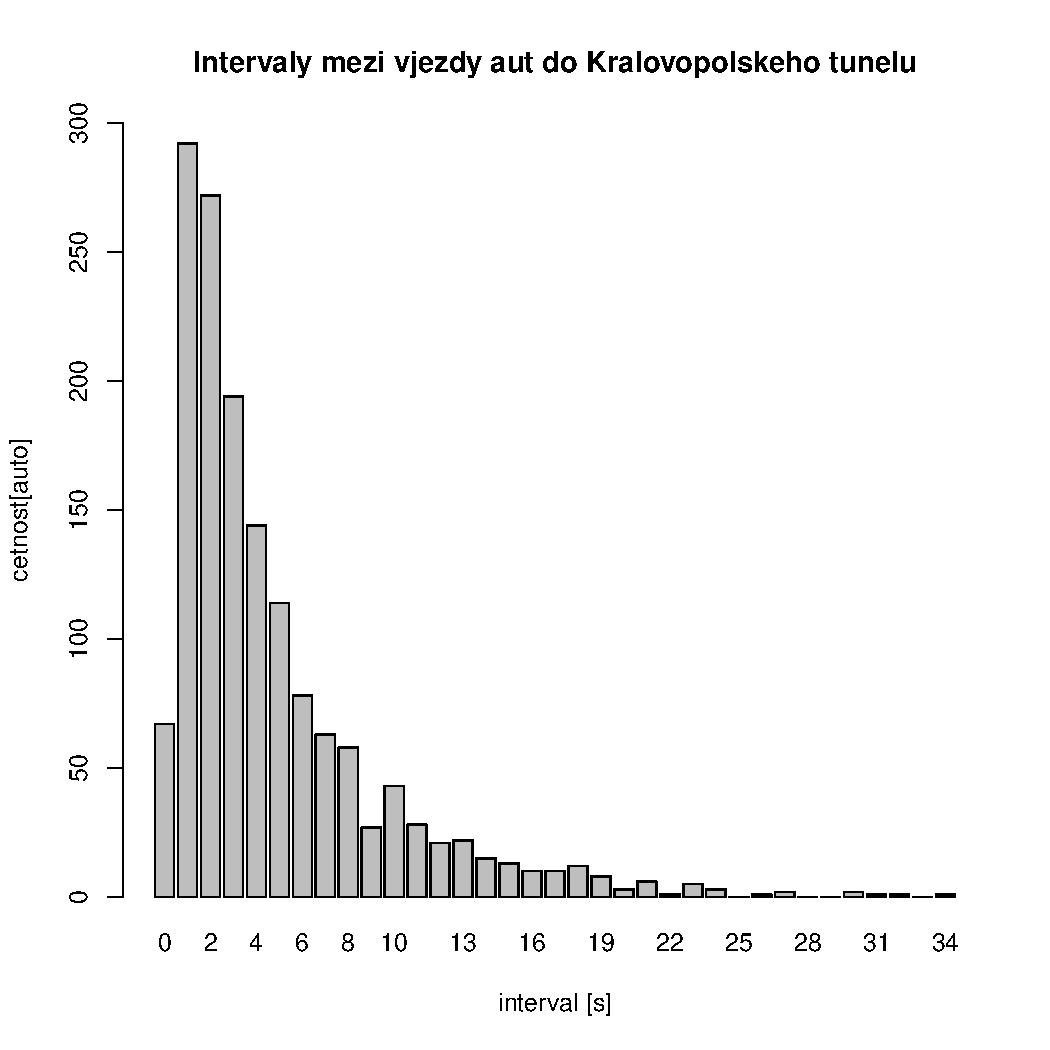
\includegraphics[width=90mm]{../measuring/tunelBarPlot.pdf}
		\caption{Histogram měření}
		\label{tunel}
		\end{figure}

	\subsection{Četnosti příchodů zákazníků na poštu Brno 12 v průběhu pracovního dne}
		\subsubsection{Měřený jev}
		Druhý jev, který jsme v rámci projektu zpracovali, jsou četnosti příchodů zákazníků na poštu 
		Brno 12 na Mojmírově náměstí v Králově Poli. Zákazník se do datového souboru zařadí v okamžiku,
		kdy si vezme pořadový lísteček z vyvolávacího systému. \\ \\
		Pracovní den jsme rozdělili do 21 intervalů pokrývajících celou otvírací dobu pošty (8.00 - 18.30),
		kdy každý interval má délku 30 minut. Měření bylo provedeno v pondělí 11.11.2013, které je dle slov
		pana Křepely vždy nejfrekventovanější den pracovního týdne.

		\subsubsection{Způsob měření}
		Měření bylo provedeno zcela automaticky vyvolávacím systémem, který o každém požadavku zaznamenává
		přesný čas zmáčknutí tlačítka (v sekundách). Mezi každodenní výstupy vyvolávacího systému patří 
		tabulka obsahující 30minutové intervaly a počty zákazníků, kteří v daných intervalech přišli. Tuto
		tabulku nám Česká Pošta byla ochotna poskytnout.


		\subsubsection{Zpracování naměřených dat}
		Tištěnou tabulku získanou od České Pošty jsme převedli do elektronické podoby a v prostředí
		R Studio jsme ji převedli na histogram zobrazený v obrázku \ref{posta} a s ním jsme dále pracovali
		při hledání rozložení klientů během dne. V histogramu jsou jednotlivé intervaly popsány počátečními časy
		jednotlivých intervalů.

		\begin{figure}[ht!]
		\centering
		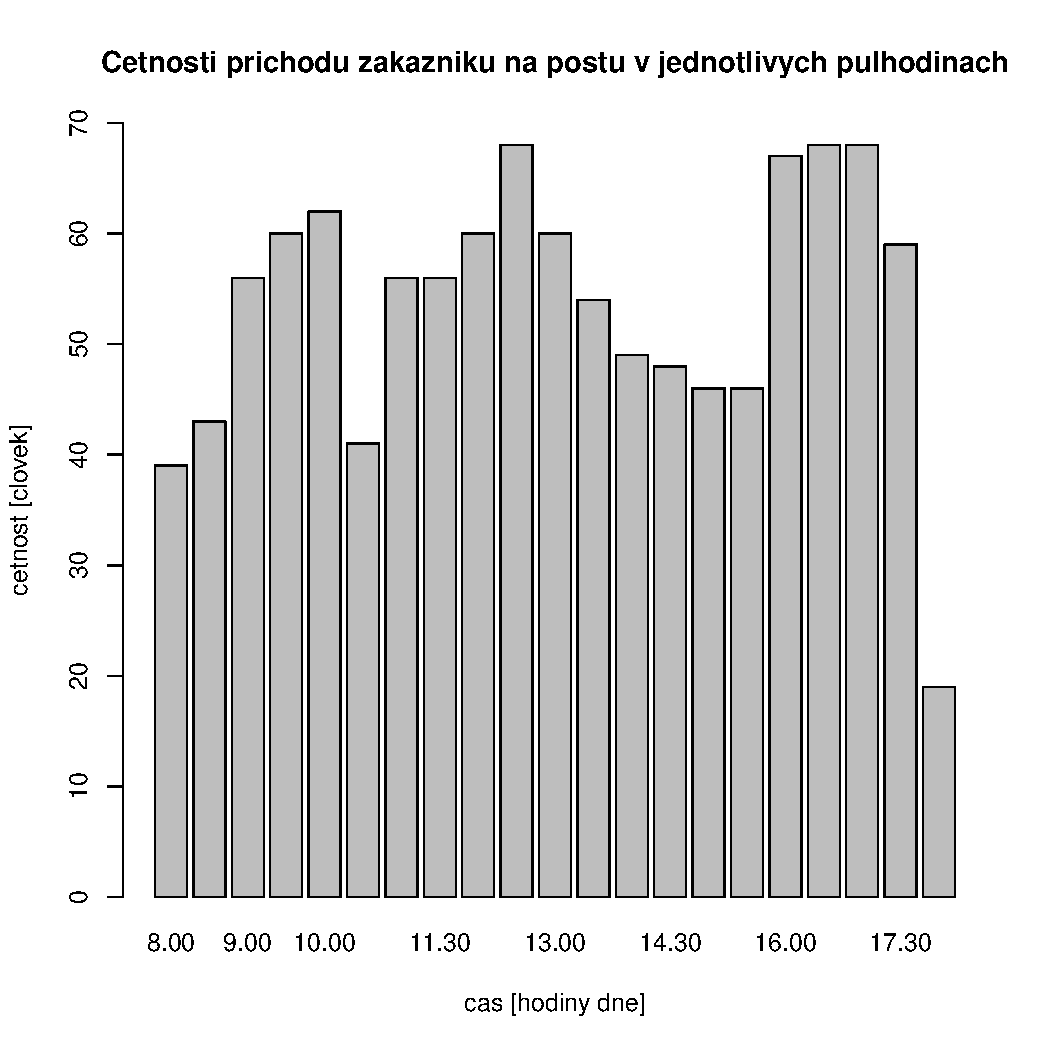
\includegraphics[width=90mm]{../measuring/postaBarPlot.pdf}
		\caption{Histogram měření}
		\label{posta}
		\end{figure}

	\subsection{Četnosti příjezdů nákladních automobilů do skladu během pracovního dne}
		\subsubsection{Měřený jev}
		Posledním z našich jevů jsou četnosti příjezdů nákladních automobilů do skladu firmy působící 
		ve Zlínském kraji, která ale bohužel nechtěla být jmenována. Tyto četnosti byly měřeny na vrátnici 
		dané firmy ve středu 27.11.2013 během celého dne (od půlnoci do půlnoci). Tato vrátnice je jedinnou
		cestou do areálu firmy, takže vypovídající hodnota našeho měření pro střed týdne by měla být 100\%. 

		\subsubsection{Způsob měření}
		U nákladních automobilů se standardně zapisuje čas příjezdu a čas odjezdu. Statistika, kterou nám firma
		poskytla seskupovala vždy počet přijíždějících nákladních aut během 60minutového intervalu. Výsledkem měření
		tedy jsou počty přijíždějících automobilů v jednotlivých hodinách dne.

		\subsubsection{Zpracování naměřených dat}
		Naměřená data jsme získali v psané podobě, převedli jsme je tedy do podoby elektronické a stejně jako v ostatních
		případech jsme si v R Studiu vykreslili histogram četností jednotlivých hodnot (Obrázek \ref{sklad}) a provedli jsme 
		teoretické prokládání histogramu funkcí hustoty pravděpodobnosti daného rozložení.

		\begin{figure}[ht!]
		\centering
		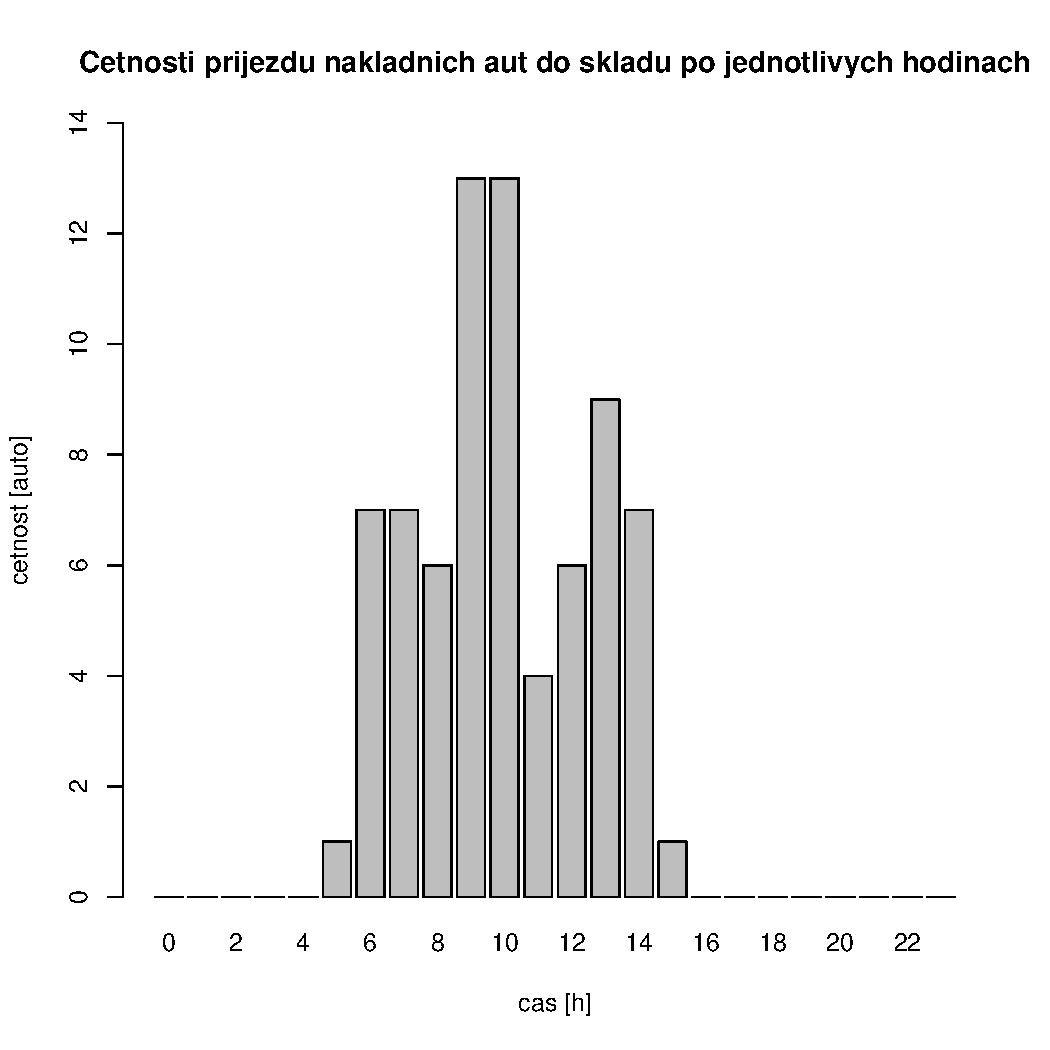
\includegraphics[width=90mm]{../measuring/skladBarPlot.pdf}
		\caption{Histogram měření}
		\label{sklad}
		\end{figure}

\section{Způsob řešení}
V této kapitole se budeme věnovat způsobu, jakým jsme dosáhli exaktních aproximací jedntolivých jevů 
reálného světa pomocí matematických funkcí hustoty rozložení. Pro naše řešení jsme využívali pouze rozložení
dostupná v knihovně SIMLIB v. 3.02 a jejich kombinace.

	\subsection{Aproximace funkcí hustoty pravděpodobnosti} 
	Každý histogram jsme tvarově porovnali s obecnými tvary funkcí hustoty pravděpodobnosti. Pokud byl tvar histogramu pro
	různé části časové osy rozdílný, rozdělili jsme ji na několik částí a v těchto částech jsme potom prováděli aproximaci 
	odděleně. V implementaci jsme tyto jednotlivé části složili dohromady takovým způsobem, že při každém generování požadavku 
	se použilo právě jedno z odvozených rozložení. Rozhodování mezi použitými rozloženími bylo prováděno s pomocí vestavěné
	funkce Random() v závislosti na tom, jaká část (v \%) naměřených hodnot patřila do danou funkcí aproximovaného intervalu.



\section{Testování}
	\subsection{Postup experimentování a okolnosti}
	Hlavní částí přesné aproximace změřeného jevu bylo testování. Po teoretickém proložení histogramu funkcí hustoty pravděpodobnosti jsme získali pro každý jev cca tři vyhovující varianty aproximace. Během testování jsme program opakovaně spouštěli a porovnávali jeho
	výsledky vynesené do histogramu s histogramy reálně naměřených jevů. Tímto způsobem jsme vždy vybrali nejvhodnější z teoretických
	aproximací a tu jsme potom experimentálně upravovali pro dosažení přesnějších výsledků. \\ \\
	Parametry, které byly nejčastěji během testování v rozloženích měněny:
	\begin{itemize}
		\item \textbf{Charakteristiky polohy} - funkce jsme posouvali jak přičítáním konstanty k výsledku, tak pomocí parametrů jednotlivých 
		funkcí (např. střední hodnota u exponenciálního rozložení nebo horní a dolní mez u rovnoměrného rozložení)
		\item \textbf{Charakteristiky variability a špičatosti}
	\end{itemize}
	\subsection{Závěr experimentů}
		\subsubsection{Intervaly mezi vjezdy jednotlivých automobilů do Královopolského tunelu}
		Po aproximaci histogramu naměřených hodnot pomocí kombinace rozložení Gama, jehož počátek byl posunut
		do hodnoty 1 a doplnění 4.6\% aut, která vjela do tunelu speciálním způsobem - zároveň s jiným autem - 
		pomocí rovnoměrného rozložení v intervalu <0,1> jsme získali graf zobrazený na obrázku \ref{genTunel}. Můžeme zde
		pozorovat aproximací s minimální chybou. O přesnosti aproximace mluví také fakt, že pokud jsme simulaci nechali běžet
		dvě hodiny modelového času, bylo vygenerováno v průměru 1537 aut oproti 1517 autům při dvouhodinovém měření.

		\begin{figure}[ht!]
		\centering
		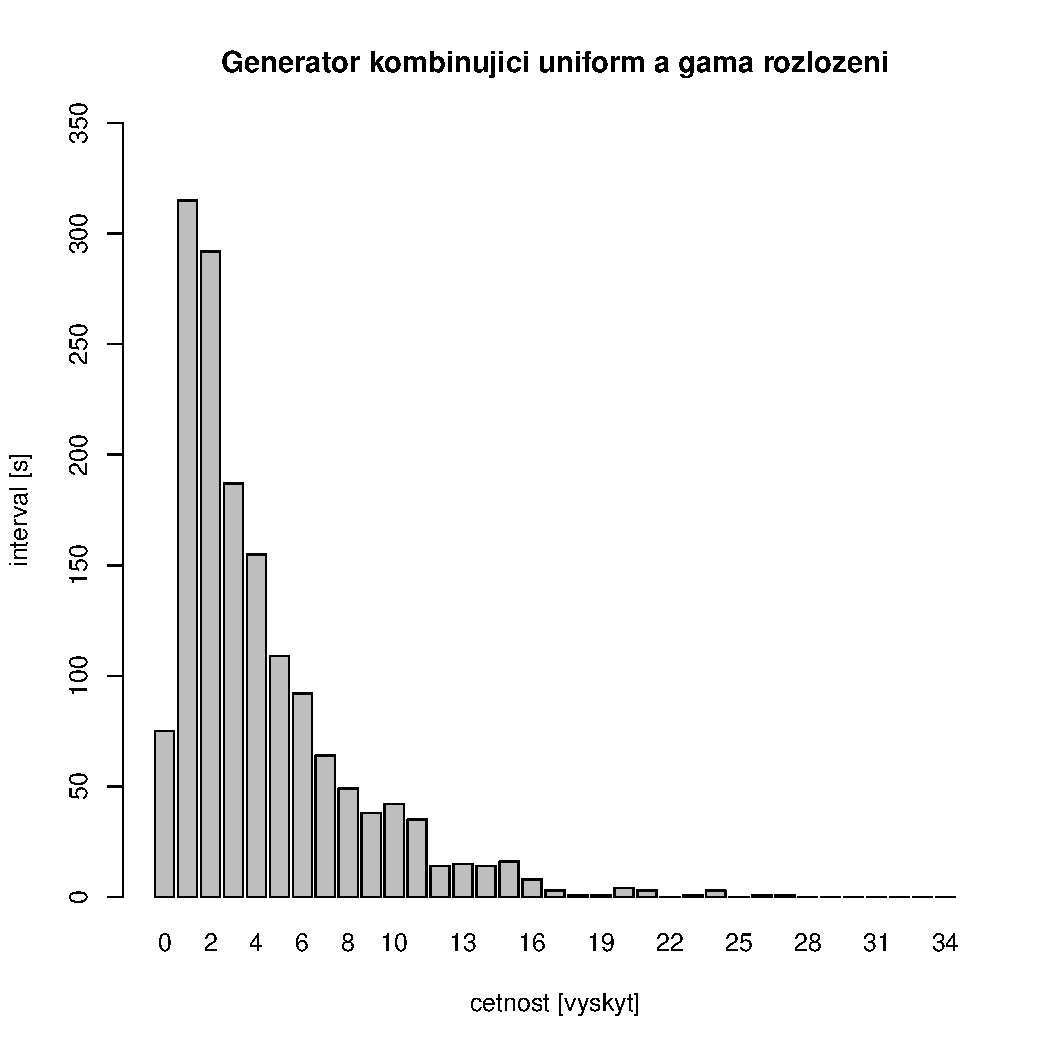
\includegraphics[width=90mm]{../measuring/generatorTunelBarPlot.pdf}
		\caption{Histogram z jednoho běhu generátoru pro tunel}
		\label{genTunel}
		\end{figure}

		\subsubsection{Četnosti příchodů zákazníků na poštu Brno 12 v průběhu pracovního dne}
		Výsledné rozložení jsme složili ze čtyř různých rozložení, ve výsledku se nám tedy objevuje dvakrát rozložení Beta a dvakrát rozložení Gama. Histogram výsledků jednoho z běhů je zobrazen na obrázku \ref{genPosta}. Lze z něj vyčíst o něco menší, stále však pro model dostačující přesnost. Soustředit bychom se tady měli hlavně na tvar výsledného histogramu, který zhruba odpovídá skutečnosti.

		\begin{figure}[ht!]
		\centering
		\includegraphics[width=90mm]{../measuring/generatorPostaBarPlot.pdf}
		\caption{Histogram z jednoho běhu generátoru pro poštu}
		\label{genPosta}
		\end{figure}	

		\subsubsection{Četnosti příjezdů nákladních automobilů do skladu během pracovního dne}	
		Při hledání vhodné aproximace jsme opět zvolili metodu rozdělit rozložení na několik samostatných rozložení, kdy jsme okrajové hodnoty modelovali pomocí normálního rozložení a maximální hodnoty pomocí rozložení rovnoměrného. Histogram výsledků je zobrazen na obrázku \ref{genSklad}. Jeho tvar i hodnoty v jednotlivých hodinách odpovídají hledanému jevu znázorněném v obrázku \ref{sklad}.

		\begin{figure}[ht!]
		\centering
		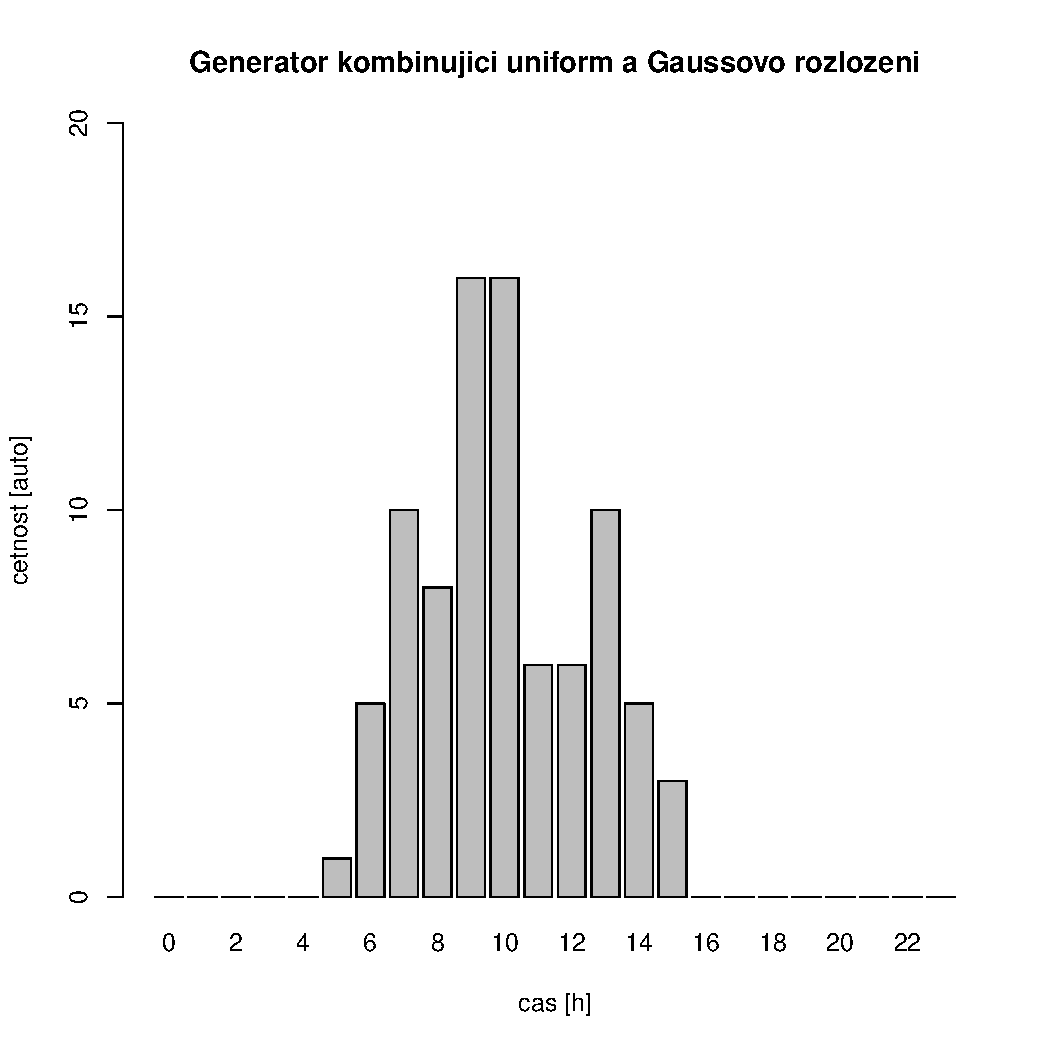
\includegraphics[width=90mm]{../measuring/generatorSkladBarPlot.pdf}
		\caption{Histogram z jednoho běhu generátoru pro sklad}
		\label{genSklad}
		\end{figure}		

\section{Závěr}
Během řešení této práce se nám povedlo nasimulovat náhodnost jevů probíhajících v reálném světě pomocí generátorů 
pseudonáhodných čísel. Dokázali jsme tím tedy, že matematický aparát generování pseudonáhodných čísel je dostatečně
flexibilní na to, aby jeho prostřednictvím bylo možné aproximovat i jevy, které na první pohled nejsou učebnicovým příkladem 
nám známých rozložení. Matematika definuje mnohem více různých rozložení než bylo uvažováno a využíváno v rámci řešeného 
projektu, proto tedy na závěr této práce můžeme prohlásit, že jakákoliv struktura reálných hodnot se dá do simulačních
modelů nahradit méně či více složitým generátorem pseudonáhodných čísel s aproximovaným rozložením.

\end{document}
